\documentclass[notes]{beamer}
\usepackage[latin1]{inputenc}
\usepackage{tikz}
\usetikzlibrary{arrows}
\usetikzlibrary{shapes.misc}
\usepackage{verbatim}
\usetheme{Warsaw}

\title{Homogeneity is Independent from Randomness}
\author{Li Ling Ko}
\institute{University of Notre Dame}
\date{22 January, 2018}
\setbeamertemplate{footline}[frame number]
\setbeamertemplate{theorems}[numbered]

\newcommand{\TODO}[1]{\textcolor{red}{TODO: #1}}
\newtheorem{thm}{Theorem}
\newtheorem{coro}{Corollary}
\newtheorem{pf}{Proof}
\newtheorem{define}{Definition}

\begin{document}
\begin{frame}
  \titlepage
\end{frame}

\begin{frame}{Ramsey's Theorem ($\text{RT}$)}
  \begin{itemize}
    \item State $\text{RT}_k^n$
    \item $\text{RT}$ is $(\forall n)\; \text{RT}_{<\infty}^n$
  \end{itemize}

  \begin{itemize}
    \item Asserts existence of homogeneity
  \end{itemize}
\end{frame}

\begin{frame}{Randomness}
  \begin{itemize}
    \item What is 1-random
    \item Lebesgue Measure
  \end{itemize}
\end{frame}

\begin{frame}{Strongly Omnisciently Computably Reducible
  ($\leq_{\text{soc}}$)}
  \begin{itemize}
    \item Define problem, solution
    \item Define $\leq_{\text{soc}}$ on WWKL, RT
  \end{itemize}
\end{frame}

\note{
  \begin{itemize}
    \item Mention other reductions
    \item soc doesn't require the second problem to be computable from the
      first one
  \end{itemize}
}

\begin{frame}{RT, KL, WKL, WWKL under $\leq_{\text{soc}}$}
  \begin{itemize}
    \item Homogeneity ``independent from'' Randomness
  \end{itemize}

  \begin{center}
    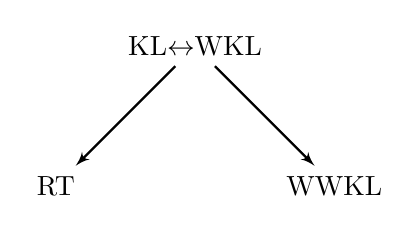
\begin{tikzpicture}[node distance=2.5cm,auto,thick,>=latex']
      \node (KL) {KL$\leftrightarrow$WKL};
      \node (WWKL) [below right of=KL] {WWKL};
      \node (RT) [below left of=KL] {RT};
      \draw[->] (KL) -- (RT);
      \draw[->] (KL) -- (WWKL);
      %\draw [->,red] (RT) -- coordinate (m) (WWKL);
      %\draw[shift={(m)},red](-0.1,-0.1)--(0.1,+0.1);
    \end{tikzpicture}
  \end{center}
\end{frame}

\begin{frame}{KL $\equiv_{\text{soc}}$ WKL}
  \begin{itemize}
    \item WKL $\leq_{\text{soc}}$ KL: From definition.
    \item KL $\leq_{\text{soc}}$ WKL: Given KL instance \textbf{P}, at
      each level, code branches into WKL instance \textbf{Q} using binary
      representation of branch number
  \end{itemize}
\end{frame}

\begin{frame}{RT $\leq_{\text{soc}}$ WKL}
  \begin{itemize}
    \item Fix $k$-coloring $c:[\omega]^n\rightarrow k$
    \item Define binary tree $T\subseteq 2^{<\omega}$ by $\sigma\in T$
      iff $\{n:\sigma(n)=1\}$ is homogeneous
  \end{itemize}
\end{frame}

\begin{frame}{WWKL $\lneq_{\text{soc}}$ WKL}
  \begin{itemize}
    \item WWKL $\leq_{\text{soc}}$ WKL: From definition.
    \item WKL $\nleq_{\text{soc}}$ WWKL: Fix instance of WKL with only one
      solution $f$, which is non-computable
    \item Set of oracles computing $f$ has 0 measure
    \item Given arbitrary instance of WWKL, since set of solutions has
      positive measure, there must be solutions that do not compute $f$ 
  \end{itemize}
\end{frame}

\begin{frame}{RT $\nleq_{\text{soc}}$ WWKL}
  \begin{itemize}
    \item $\text{RT}_2^1$ $\nleq_{\text{soc}}$ WWKL
    \item Fix $A\in[\omega]^\omega$ where
      \begin{align*}
        &\mu(\{X: X\; \text{computes an element in}\; [A]^\omega\}) =0,\\
        \text{and}\;\;\; &\mu(\{X: X\; \text{computes an element in}\;
        [\bar{A}]^\omega\}) =0.\\
      \end{align*}
    \item Choose 2-coloring $c:\omega\rightarrow\{0,1\}$, $c(n)=0
      \Leftrightarrow n\in A$.
    \item Given any instance of WWKL, since the set of its paths has
      measure $>0$, some path must fail to compute any infinite
      homogeneous set of $c$. 
    \item Bi-hyperimmune sets $A$ work.
  \end{itemize}
\end{frame}

\begin{frame}{$A$ Hyperimmune $\implies \mu(\{X: X\; \text{computes an
element in}\; [A]^\omega\}) =0$}
  Hyperimmune sets $A$ are characterized as those whose principal
  function $p_A$ is not dominated by any recursive $f$. \\
  \vspace{1em}

  Bi-Hyperimmune sets $A$ are those where $A$, $\bar{A}$ are hyperimmune.\\
  \vspace{1em}

  \textbf{Main idea:} Assume not. Then there are enough paths computing
  infinite subsets of $A$ such that we can effectively ask them to ``vote''
  for when new elements of $A$ have appeared. Thus giving recursive
  $f$ that dominates $p_A$.\\
  \vspace{1em}

  Fix Turing functional $\Phi$. Write $\mathcal{C} :=\{X:
  \Phi^X\in[A]^\omega\}$. Note $\mathcal{C}$ is Borel and thus measurable.
  Since the measure of a countable union of null sets is 0, and
  there are only countably many Turing functionals, it suffices to show
  $\mu(\mathcal{C})=0$. Assume $\mu(\mathcal{C})=4m>0$.
\end{frame}

\begin{frame}{$A$ Hyperimmune $\implies \mu(\{X: X\; \text{computes an
element in}\; [A]^\omega\}) =0$ (cont.)}
  \begin{itemize}
    \item Approximate $\mathcal{C}$ by open cover
      $\mathcal{O}\supseteq\mathcal{C}$ with
      $\mu(\mathcal{O}-\mathcal{C})<m$.
    \item Approximate $\mathcal{O}$ by basic open sets
      $[\sigma_0],\ldots,[\sigma_n] \subseteq\mathcal{O}$ with
      \[\mu(\mathcal{O}-([\sigma_0]\cup\ldots\cup[\sigma_n])) <m.\]
    \item Fix effective enumeration of branches $\sigma$ in
      $[\sigma_0]\cup\ldots\cup[\sigma_n]$.
    \item At stage $s=0$, wait till a measure of $2m$ of such $\sigma$'s
      finds an element via $\Phi$; let $f(0)$ be the largest element found.
      Since $[\sigma_0]\cup\ldots\cup[\sigma_n]$ approximate $\mathcal{C}$
      tightly, such $\sigma$'s exist, and more than a measure of $m$ of
      them indeed lie in $\mathcal{C}$.
    \item In particular, at least one of these $\sigma$'s really computes
      an infinite subset of $A$, so $f(0)\geq p_A(0)$.
    \item At stage $s+1$, wait till a measure of $2m$ of $\sigma$'s
      finds an element exceeding $f(s)$; let $f(s+1)$ be the largest
      element found.
  \end{itemize}
\end{frame}

\begin{frame}{Bi-Hyperimmune sets $A$ exist}
  \begin{itemize}
    \item Want $A$ where $p_A,p_{\bar{A}}\not<f$ for all recursive $f$.
    \item Fix $\emptyset''$-enumeration $f_0,f_1,\ldots$ of all recursive
      functions.
    \item At stage $n$, we have defined the first $i$th elements of $A$.
    \item Put enough elements into $\bar{A}$ so that the $(i+1)$th element
      of $A$ exceeds that of $f_n$.
    \item Then we would have defined the first $j$th elements of $\bar{A}$.
    \item Similarly, put enough elements into $A$ so that the $(j+1)$th
      element of $\bar{A}$ exceeds that of $f_n$.
  \end{itemize}
\end{frame}

\begin{frame}{Characterizing $\Pi_1^0$-encodable
$\mathcal{C}\subseteq\omega^\omega$}
  For the remaining directions
  \begin{itemize}
    \item WKL $\nleq_{\text{soc}}$ RT
    \item WWKL $\nleq_{\text{soc}}$ RT
  \end{itemize}

  we need the following definition and characterization:
  \begin{define}[$\Pi_1^0$-encodability]
    $\mathcal{C}\subseteq \omega^{\omega}$ is $\Pi_1^0$-encodable if
    \TODO{write out definition}.
  \end{define}

  \begin{thm}[Characterizing $\Pi_1^0$-encodable
  $\mathcal{C}\subseteq\omega^\omega$]
    $\mathcal{C}\subseteq \omega^{\omega}$ compact. Then
    \[\mathcal{C}\; \text{is}\; \Pi_1^0\text{-encodable}\; \Leftrightarrow
    \mathcal{C}\; \text{contains non-empty}\; \Sigma_1^1\; \text{subset}.\]
  \end{thm}
\end{frame}

\begin{frame}{Characterizing Recursively-Encodable $A\subseteq\omega$}
  \begin{define}[Recursive-Encodability]
    $A\subseteq\omega$ is recursively-encodable if given any
    $X\in[\omega]^\omega$, some subset of $X$ computes $A$.
  \end{define}

  \begin{coro}[Characterizing Recursively-Encodable $A\subseteq\omega$]
    $A\subseteq\omega$ is recursively-encodable if and only if it is
    hyperarithmetic.
  \end{coro}
\end{frame}

\begin{frame}{WKL $\nleq_{\text{soc}}$ RT}
  \begin{itemize}
    \item Fix instance of WKL with only one solution $f$, which is
      not hyperarithmetic
    \item Fix instance \textbf{Q} of RT, assume by contradiction all
      its solutions compute $f$ 
    \item Given arbitrary $X\in[\omega]^\omega$, relativize \textbf{Q} to
      $X$, there exists some homogeneous $Y\in[X]^\omega$
    \item By assumption, $Y$ computes $f$. Since $X$ is arbitrary, $f$ is
      computably encodable.
    \item But being computably encodable is the same as being
      hyperarithmetic, $\rightarrow\leftarrow$.
  \end{itemize}
\end{frame}

\begin{frame}{WWKL $\nleq_{\text{soc}}$ RT}
  \begin{itemize}
    \item Fix $T\subseteq 2^{<\omega}$ with $\mu(T)>0$, $[T]$
      has no non-empty $\Sigma_1^1$ subset
    \item We prove such $T$ exists
    \item Fix RT instance $c:[\omega]^n\rightarrow k$ and assume every
      solution $H$ computes a path through $T$, i.e. $[T]$ has non-empty
      $\Pi_1^{0,H}$ subset
    \item Thus every $X\in[\omega]^\omega$ has a subset
      $H\in[X]^\omega$ such that $[T]$ has non-empty $\Pi_1^{0,H}$ subset
    \item We say that $T$ is $\Pi_1^0$-encodable
    \item We will prove that being $\Pi_1^0$-encodable is equivalent to
      containing non-empty $\Sigma_1^1$ subset, $\rightarrow\leftarrow$
  \end{itemize}
\end{frame}

\begin{frame}{There exists $[T]$ with no $\Sigma_1^1$ subset, $\mu(T)>0$}
  \begin{itemize}
    \item Let $T$ be set of Martin-Lof randoms relativized to Kleene's $O$
    \item Then $\mu(T)>0$
    \item $T$ has no non-empty $\Sigma_1^1$ subset because every
      $\Sigma_1^1$ subset of $2^\omega$ contains an element recursive in
      $O$
  \end{itemize}
\end{frame}

\begin{frame}{Easy: Contains non-empty $\Sigma_1^1$ subset $\rightarrow$
$\Pi_1^0$-encodable}
  \newtheorem{main-easy}{Easy direction}
  \begin{main-easy}
    $\mathcal{C}\subseteq \omega^{\omega}$ compact.

    $\mathcal{C}$ contains non-empty $\Sigma_1^1$ subset
    $\rightarrow$

    $\mathcal{C}$ is $\Pi_1^0$-encodable.
  \end{main-easy}

  \newtheorem{pf-easy}{Proof}
  \begin{pf-easy}
    Contain $\Sigma_1^1$ subset $\implies$ has modulus. Given arbitrary
    $X\in[\omega]^\omega$, make $X$ sparse enough for principal function to
    dominate modulus.
  \end{pf-easy}
\end{frame}

\begin{frame}{Hard: $\Pi_1^0$-encodable $\rightarrow$ Contains
non-empty $\Sigma_1^1$ subset}
  \begin{itemize}
    \item Fix compact $\mathcal{C}$ with no non-empty $\Sigma_1^1$ subset.
      We want $G\in[\omega]^\omega$ such that no $X\in[G]^\omega$
      can compute (in the $\Pi_1^{0,X}$ sense) a non-empty subset of
      $\mathcal{C}$.

    \item Fix enumeration of Turing functionals $\Gamma_s:\omega^{<\omega}
      \rightarrow \omega^{<\omega}$.

    \item Construct $G=\bigcap_{s\in\omega}G_s$, where
      $\omega=G_0\supset G_1\supset\ldots$.
      
    \item At stage $s$, fix the first $s$ elements of $G$.
    
    \item Then remove enough elements beyond the first $s$ ones so that no
      $X\in[G_s]^\omega$ can compute a non-empty subset of $\mathcal{C}$
      via $\Gamma_s$.

    \item Then $|G|=\omega$, and $G$ satisfies the desired property.

    \item The hard part is proving such $G_{s+1}\in[G_s]^\omega$ exists.
  \end{itemize}
\end{frame}

\begin{frame}{Desired $G_{s+1}\in[G_s]^\omega$ exists}
  \begin{itemize}
    \item Fix $G_0\in[\omega]^\omega$, $n\in\omega$, compact
      $\mathcal{C}\subseteq\omega^\omega$, Turing functional
      $\Gamma:\omega^{<\omega} \rightarrow \omega^{<\omega}$.

    \item Want $G_1\in[G_0]^\omega$ such that $G_1\restriction
      n=G_0\restriction n$, and no $X\in[G_1]^\omega$ computes a non-empty
      subset of $\mathcal{C}$ via $\Gamma$.

    \item If we do not require $G_1\restriction n=G_0\restriction n$, then
      we can find $G_1$ with stronger property:
  \end{itemize}

  \newtheorem{L1}{Lemma 1}
  \begin{L1}
    Fix $G_0\in[\omega]^\omega$, compact
    $\mathcal{C}\subseteq\omega^\omega$ with no non-empty
    $\Sigma_1^{1,G_0}$ subset, Turing functional $\Gamma:\omega^{<\omega}
    \rightarrow \omega^{<\omega}$, $t\in\omega$. Then there exists
    $G_1\in[G_0]^\omega$ such that every $X\in[G_1]^\omega$ does not
    compute a non-empty subset of $\mathcal{C}$ via $\Gamma$ in the
    sense:

    \begin{itemize}
      \item Either $\mathcal{C}\cap[\Gamma^X]=\emptyset$,
      \item Or...
    \end{itemize}
  \end{L1}
\end{frame}

\begin{frame}{Desired $G_{s+1}\in[G_s]^\omega$ exists (continued)}
  \begin{itemize}
      \item Fix enumeration $\{D_0,\ldots,D_m\}$ of subsets of
        $G_0\restriction n$

      \item Apply Lemma 1 $m$ times, once for each $D_i$.
  \end{itemize}
\end{frame}

\begin{frame}{Lemma 1}
  \begin{itemize}
    \item Proving Lemma 1 uses $\Sigma_1^1$-immunity basis theorem and
      Galvin-Prikry
  \end{itemize}
\end{frame}

\begin{frame}{$\Sigma_1^1$-immunity basis theorem}
  \begin{itemize}
    \item Proving this theorem uses fact that relativized Gandy-Harrington
      topoloty is Baire space
  \end{itemize}
\end{frame}

\begin{frame}{Possible backup slides}
  \begin{itemize}
    \item Set of oracles computing a fixed non-recursive has 0 measure
    \item Gandy-Harrington topology (relativized) is Baire
  \end{itemize}
\end{frame}

\begin{frame}{\textcolor{red}{Possible backup slides (reading)}}
  \begin{itemize}
    \item Every $\Sigma_1^1$ subset of $2^\omega$ contains an element
      recursive in Kleene's $O$
    \item If $A$ is hyperimmune, then set of oracles that compute
      infinite subsets of $A$ has 0 measure [Mileti]
    \item Galvin-Prikry
    \item Being encodable characterizes HYP
  \end{itemize}
\end{frame}
\end{document}
